\chapter{LEGEND}\label{chap:legend}

LEGEND used the best technologies, and existing resources, from {\MJMit} and GERDA to deploy a 200 kg detector array in the GERDA cryostat (L200). LEGEND aims to pursue a tonne-scale \geEn{} experiment in the next phase of its experimental program (L1000), with $0\nu\beta\beta$ discovery potential at a half-life approaching or at $10^{28}$ years \cite{LEGEND2021}. 

\section{A Trans-Atlantic Union}

GERDA and {\MJMit} have the lowest and second-lowest background rates and second-best and best energy resolutions of any \novbb{} experiment respectively.

The {\MJDEMit}'s careful study and selection of radiopure construction materials resulted in ultra-low background levels. In particular, {\MJMit}'s development and use of UGEFCu spearheaded this result with specific activities orders below many of the other materials employed~\cite{assaypaper}. Note that most of the mass in proximity of the detectors is UGEFCu. Another low-background component developed by the {\MJMit} collaboration is the LMFE. The LMFE sits next to the p$^+$ contact of each detector and in combination with further electronics upstream, constitutes the preamplifier for each channel. This design places the preamplifier's critical components next to the detector to avoid noise pickup along cables, and moves all the other -- often high activity -- electronics further away. The use of LMFEs was instrumental to the {\DEMit}'s record energy resolution.

By integrating the materials and electronics pioneered by the {\MJMit} collaboration into GERDA-style germanium strings in a LAr veto, the record background rate of GERDA can be surpassed. This is the strategy used by the LEGEND collaboration, driving its discovery potential to \novbb{}. From their onset, the {\MJMit} and GERDA collaborations developed joint analysis and simulation software and shared PSD techniques and Ge detector characterization results. These techniques have matured in the last decade and are ripe for their application to LEGEND data. The combination of ultra low background materials, low-noise front-end electronics, mature PSD techniques, and a LAr veto with an improved light readout system, results in a predicted background rate of $2 \times 10^{-4}$ c/(keV\,kg\,yr) and $9 \times 10^{-6}$ c/(keV\,kg\,yr) for L200 and L1000 respectively~\cite{legend_pcdr}. 

\section{L200}

Using the GERDA water tank and LAr cryostat at LNGS allowed LEGEND to expedite the deployment of a 200\,kg \geEn{} detector array. L200 utilizes the existing 70\,kg of detectors from GERDA and {\MJMit} in addition to 130\,kg of new ICPC detectors. Modifications to the GERDA infrastructure were needed to accommodate the larger L200 array. The Ge detector strings were mounted in between two new fiber optic barrels, designed specifically for the L200 string layout. The new design, in combination with higher-purity LAr, has led to higher light yield, transmission and detection. Each string consists of detector units, varying in number and size depending on the unique geometry of each detector. The detector configuration of each string and the string placement with respect to others has been optimized to increase light collection, detector density (results in more coincident events in neighboring detectors, thus allowing to discriminate against gamma backgrounds), and maintain the balance of the array. 
\begin{figure}[htb]
	\centering
	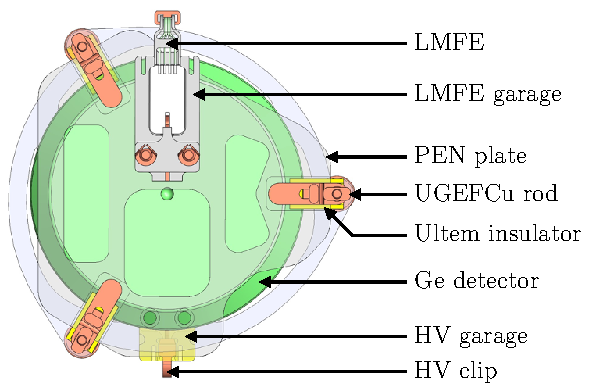
\includegraphics{figs/legend/detector_unit_width_4in.pdf}
	\caption{Render of the L200 detector unit.}
	\label{fig:legend_detector_unit}
\end{figure}

Each detector unit consists of a Polyethylene naphthalate (PEN) plate supporting three UGEFCu rods and an LMFE garage. PEN is a radiopure scintillating structural plastic~\cite{pen}, thus PEN plates increase light yield and transmission in a region proximal to the detector. The detector sits on three radiopure ultem insulators and is wire bonded to the LMFE garage. A LMFE is docked in the garage and its wires follow the string towards the top copper plate and is connected to a CC4 board, closing the preamplifier circuit. The CC4 board accommodates multiple LMFE connections. Note that this design allows LMFEs to be replaced without disassembling a string. A similar garage houses a HV clip which supplies up to 5000\,V to the detector. The detector units link and hang from one another at the UGEFCu rods forming a string. The strings are enclosed in nylon mini-shrouds. This impedes the drift of $^{42}$K ions outside the shroud volume towards the detector, thus mitigating $^{42}$K beta background in the \novbb{} ROI. However, nylon is opaque to the 128\,nm scintillation light of Ar and therefore the shrouds are coated with wavelength shifting tetra-phenyl-butadiene (TPB). The light is shifted to 450\,nm which is suitable for transmission through the mini shrouds and detection by the LAr veto~\cite{gerda_upgrade}. In similar fashion the optic fibers comprising the inner and outer fiber barrels are coated with TPB. The barrels surround the strings to maximize light collection. In each barrel, the fibers are coupled to silicon photomultipliers (SiPMs) at the top and bottom. 

The Ge array and light readout system is lowered into the center of the LAr cryostat for operation, where it is surrounded by a wavelength shifting reflector. The LAr cryostat is filled with 5N LAr, and its optical properties and thus purity are monitored by the Liquid Argon Monitoring Apparatus (LLAMA)~\cite{llama}. The LAr acts as a cooling medium for the Ge detectors, an active scintillating volume in the near detector region, and a passive high-density radiation shield. Radioactive sources are lowered into the deployed array to perform periodic energy calibrations. The sources are encapsulated and guided through the source guidance funnels and calibration source tubes to multiple locations along the Ge strings.

The LAr cryostat sits in a 8.5\,m high water tank which is filled with 590\,m$^{3}$ of ultra-pure water for operation. The 3500\,m water equivalent overburden in the LNGS underground site results in a muon flux of around $3.5\times10^{-4}$\,m$^{-2}$s$^{-1}$~\cite{lngs_muon_flux}. GERDA measured a muon rate of 0.04\,Hz~\cite{gerda_muon_veto} with the same infrastructure. The Cherenkov light created by the passage of muons in water is read out by PMTs on the walls and floor of the water tank. Coincident events in the Ge and water tank can thus be vetoed. The coincidence window in Ge is expanded to further veto prompt events proceeding a muon interaction. The resulting deadtime acquired highlights the need for a deep underground location.

L200 targets a 1\,tonne\,yr of exposure to reach a 3$\sigma$ \novbb{} discovery sensitivity of 10$^{27}$\,yr. This translates into a \mbb{} upper limit in the range of 34-78\,meV. The target exposure can be reached by operating the 200\,kg array for 5 years. The 130\,kg of new ICPC detectors have an average mass above 2\,kg, approximately twice that of the largest PPCs and BEGe detectors employed. Thus, the number of new detectors needed to reach the target exposure was halved. Fewer detector channels translates into fewer structural materials, cables and electronics in the array, thus resulting in a significant background reduction. These detectors have a lower surface to volume ratio which mitigates surface backgrounds as discussed. The combination of the adoption of {\MJMit}-style low-noise electronics, low-mass and radiopure components, a LAr veto with higher light yield and transmission, and larger detector masses results in a projected $2.5\times$ reduction from GERDA's record background index. L200 has been in a stable data-taking configuration since March 2023.
\begin{figure}[H]
	\centering
	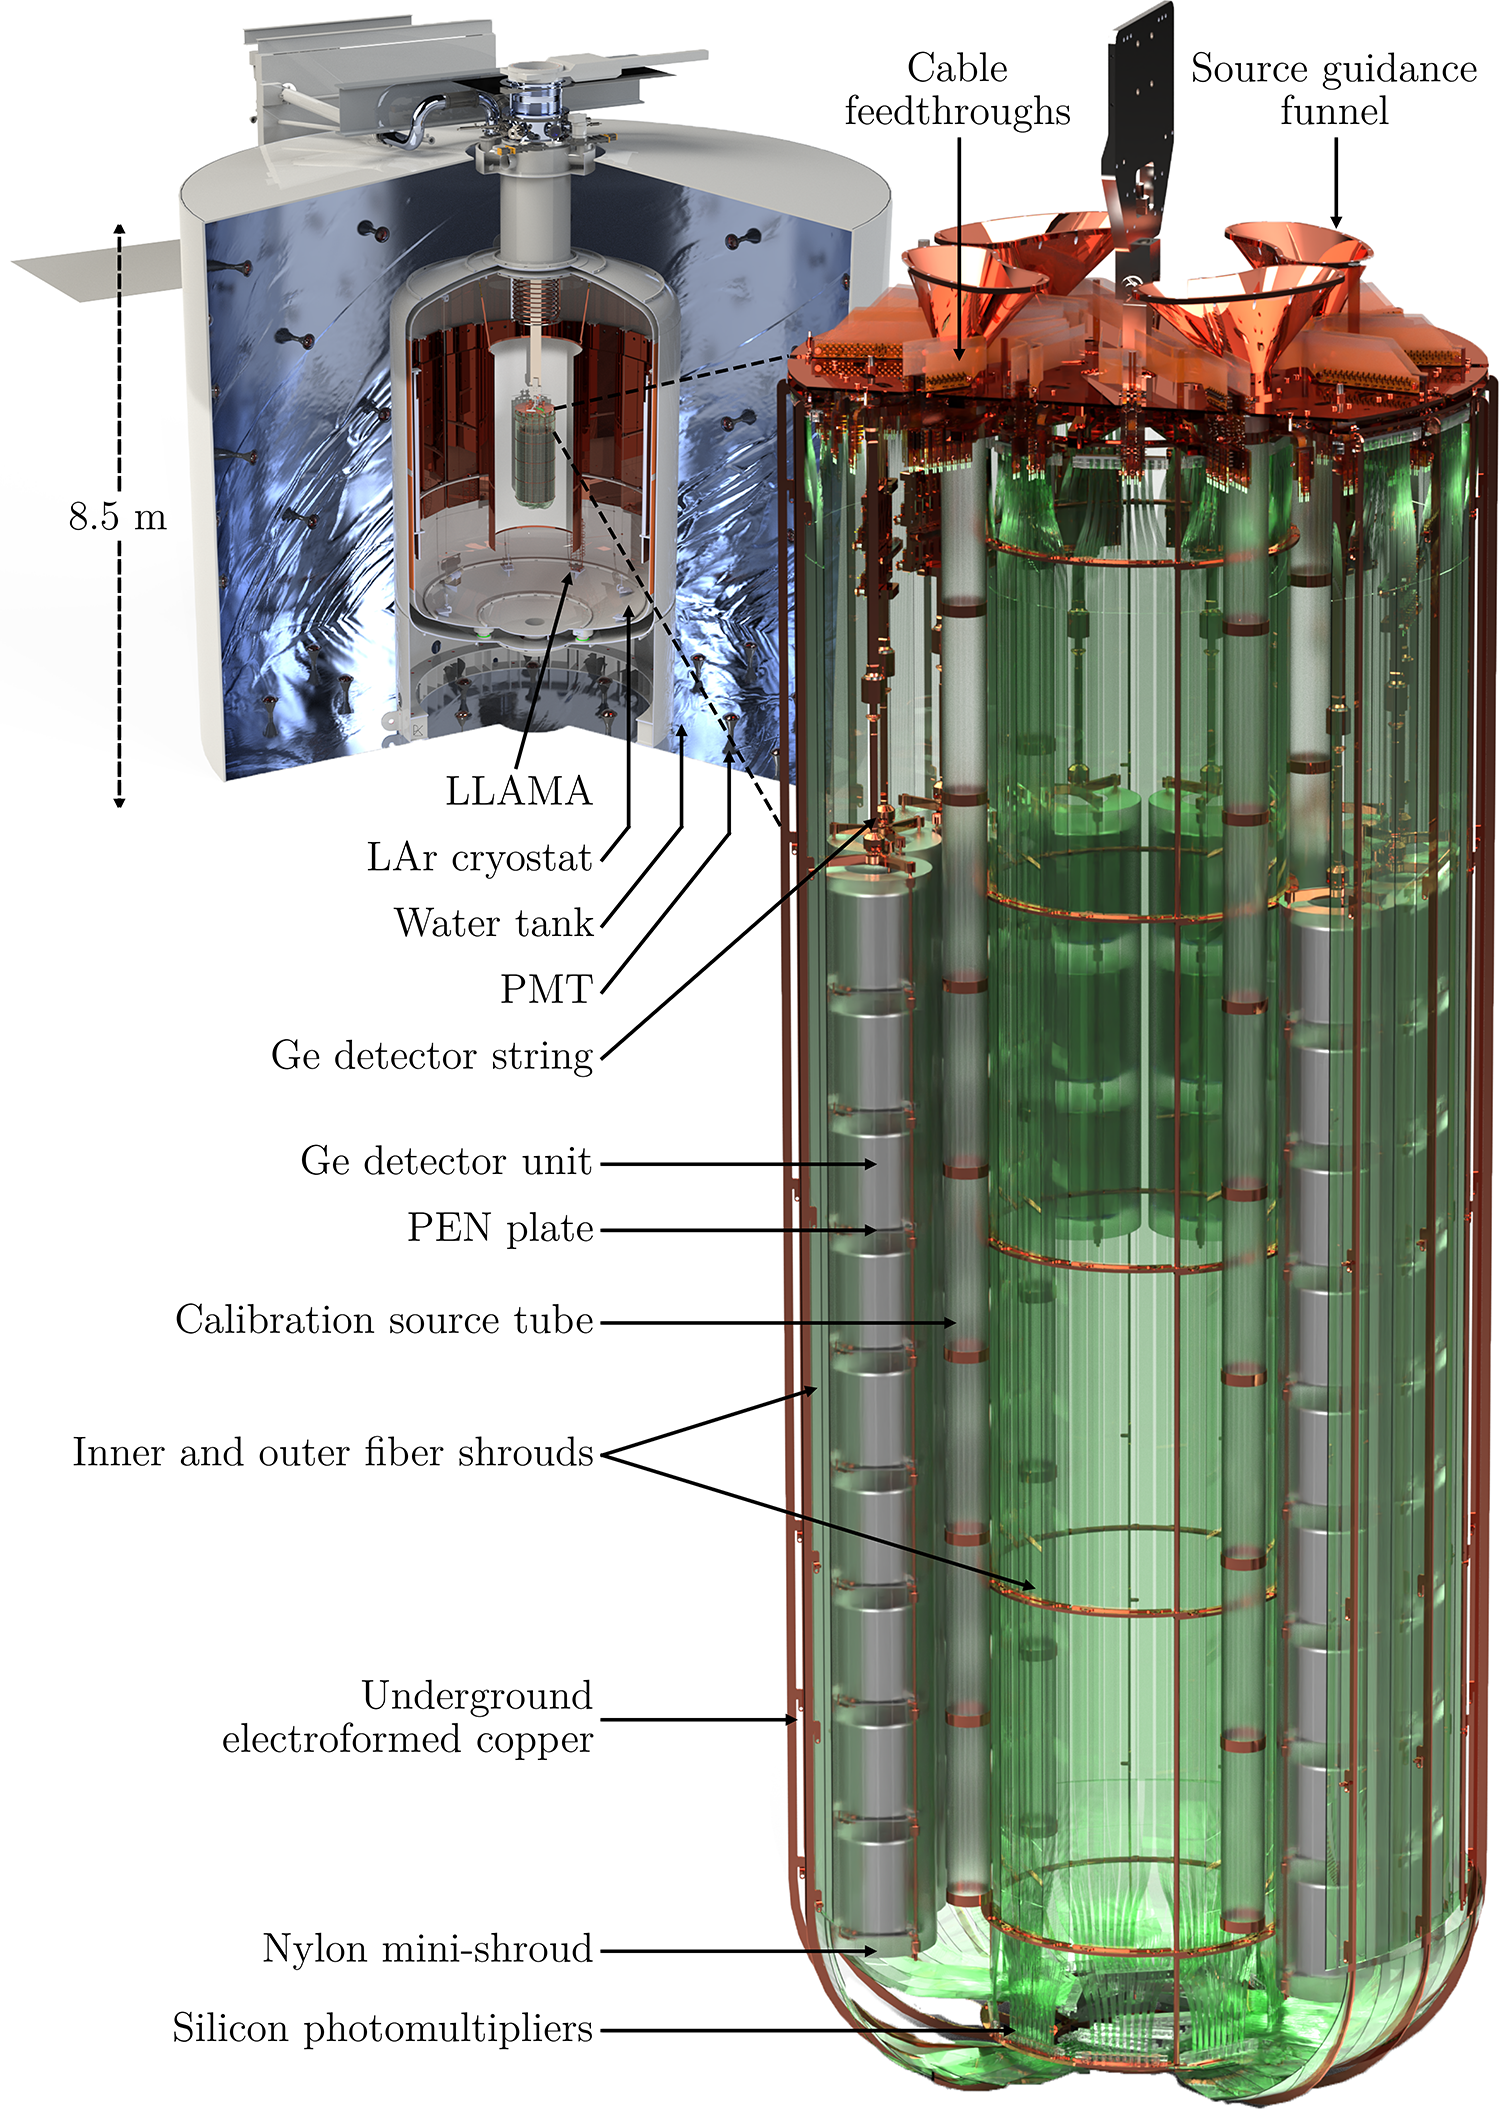
\includegraphics[width=5.4in]{figs/legend/legend_width_6in_rq.png}
	\caption{Render of the full L200 experimental design with a zoom into the Ge payload with light readout system. The front-facing Ge strings and section of the outer fiber barrel are cut out for clarity. The individual water tank and barrel schematics were rendered by Patrick Krause of the LEGEND collaboration.}
	\label{fig:legend_barrel}
\end{figure}

\section{L1000}

In the proposed L1000 experiment, 42 strings -- totaling over 1000\,kg of \geEn{} -- are operated in underground sourced LAr (UGLAr)~\cite{legend_pcdr}. The target average detector mass is 3\,kg. The UGLAr will be sourced from a deep CO$_2$ well and has been demonstrated to contain 1400 times less $^{39}$Ar than atmospheric Ar~\cite{uglar}. $^{39}$Ar and $^{42}$Ar are both produced in atmospheric Ar by cosmogenic activation, thus a similar reduction factor for $^{42}$Ar is expected. This reduction results in a drastic suppression of the $^{42}$K background in L1000 as compared to L200. The strings will be independently deployed in an UGLAr-filled reentrant UGEFCu tube, allowing payloads to be deployed as detectors are manufactured. A large atmospheric LAr cryostat houses the reentrant tube and provides additional passive shielding and light readout. The light readout system in this region is under study with PMT- and SiPM-clad walls being considered.  Similar to L200 and GERDA, the atmospheric LAr cryostat sits in a water muon-veto tank. The light readout system in the L1000 strings is similar to that of L200, but each string will have its own fiber array with improvements in light yield, transmission, and detection. The experimental site is under consideration, with LNGS as the main candidate.
\begin{figure}[htb]
	\centering
	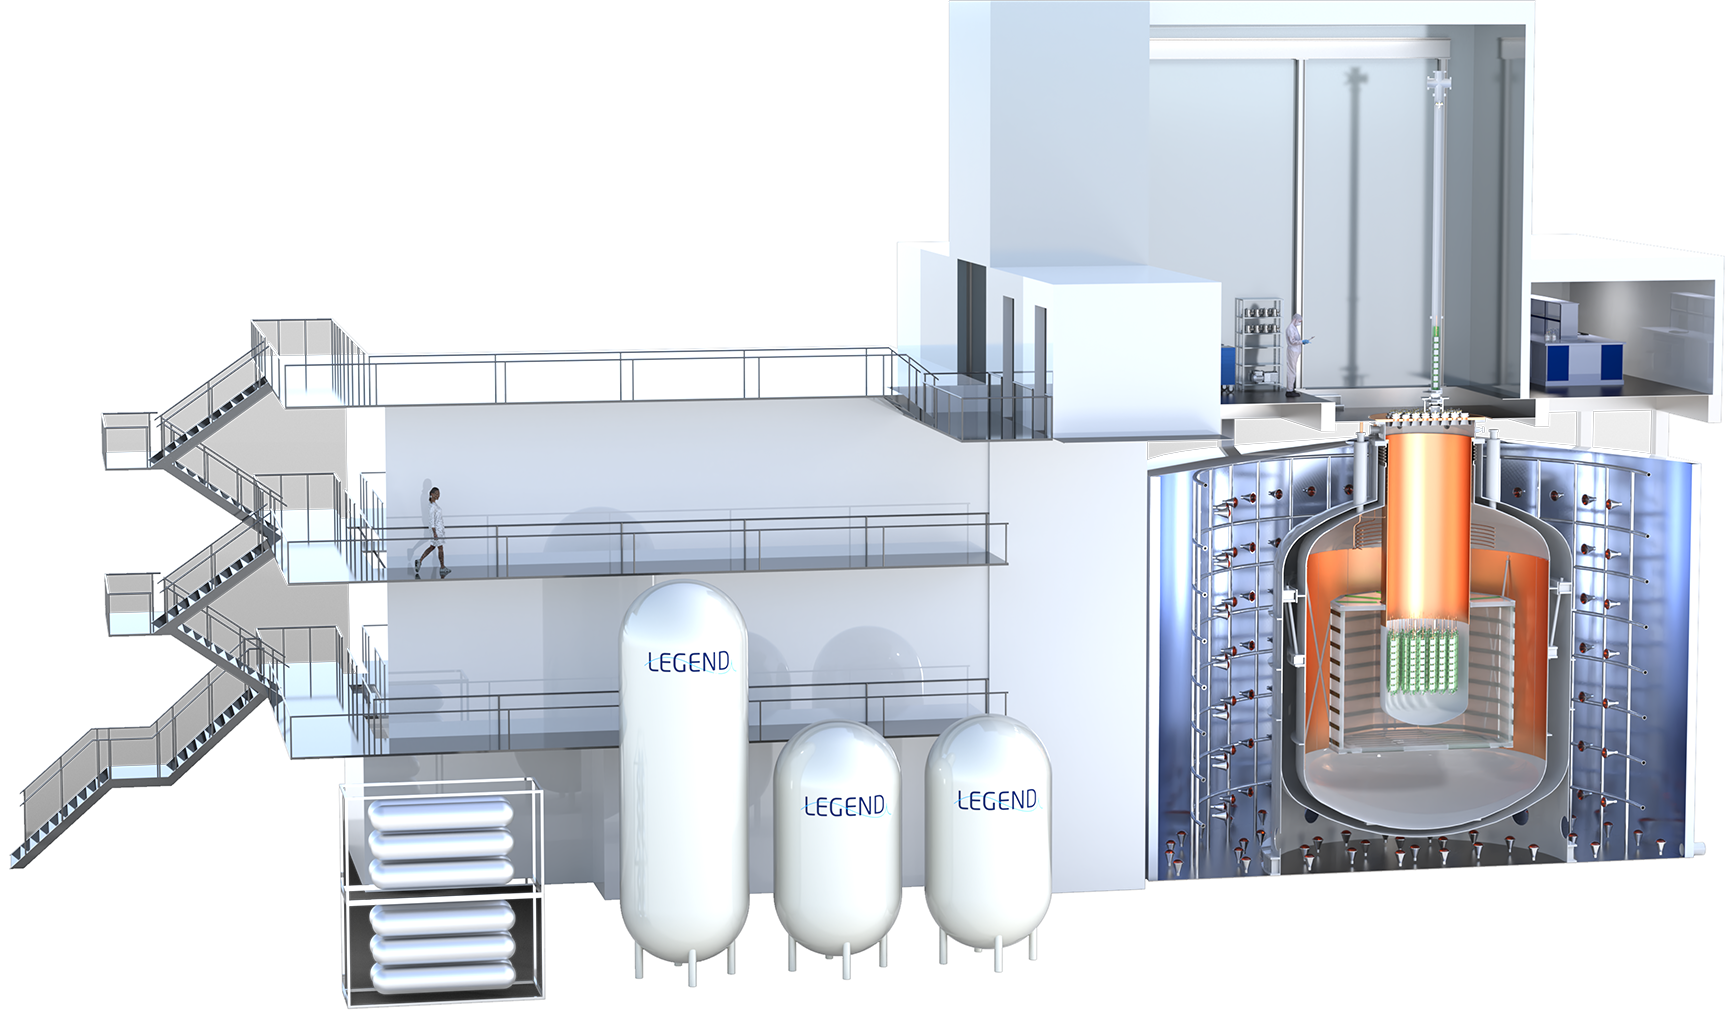
\includegraphics[width=6in]{figs/legend/L1000.png}
	\caption{The conceptual design of the L1000 experiment. Rendered by Patrick Krause.}
	\label{fig:legend1000}
\end{figure}

The detector signal readout sees a major modification from L200. Each Ge detector is wire-bonded to a front-end application-specific integrated circuit (ASIC) board. The low-background ASIC board outputs an amplified signal directly at the detector, as opposed to the approximately 1\,m long LMFE-CC4 loop. The advantage of ASIC-based front electronics is thus two-fold: besides the in-detector-unit pre-amplification, the mass and activity of the near-detector electronics is drastically reduced. Due to the design of L1000, the detector signals have to travel around 10\,m until digitized. Therefore, the use of ASICs is crucial to drive signals this distance with minimal distortion. 

The factor of over 20 reduction in background from L200 to L1000 is driven by the use of UGLAr to reduce the content of $^{42}$K. Meanwhile, the shift to ASIC-readout and the using larger detectors reduces the backgrounds originating from structural components and electronics ($^{232}$Th and $^{238}$U) and from surface alphas. The cosmogenic production of $^{68}$Ge in Ge detectors constitutes a problematic background. It undergoes electron capture to form $^{68}$Ga, which given its Q-value of 2.9\, MeV has a decay spectrum covering the \novbb{} ROI~\cite{mjd_muonic}. $^{68}$Ga decays within the detector, with an event topology that mimics that of \novbb{}; therefore, it is not possible to discriminate against these events. For this reason, the amount of time that the detectors (and raw Ge) spend on the Earth's surface is minimized and carefully monitored. The 271-day half-life of $^{68}$Ge allows for a cool-down in the live-time of the experiment. The principal projected backgrounds of L1000 (before analysis cuts, as compared to GERDA) are outlined in Fig.~\ref{fig:legend_background}. 
\begin{figure}[htb]
	\centering
	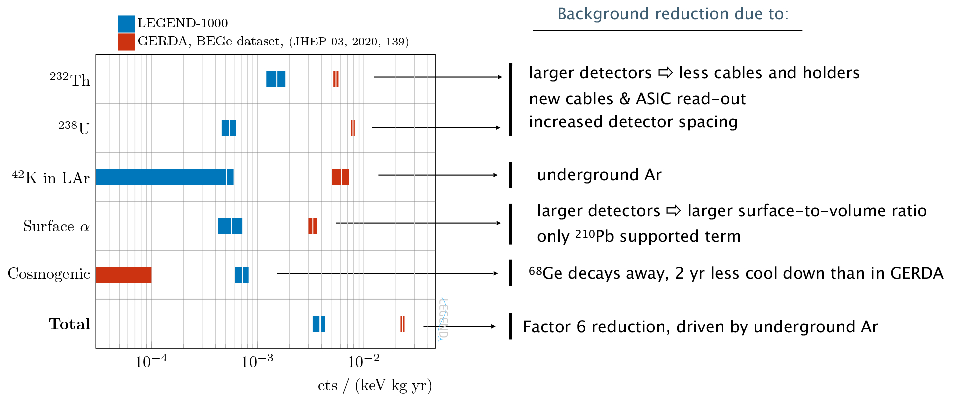
\includegraphics[width=6in]{figs/legend/legend_background.pdf}
	\caption{``The expected background index associated with each of the dominant sources, before applying analysis cuts, projected for LEGEND-1000 (blue) and measured in GERDA (red). Significant reductions in all categories, with the exception of internal cosmogenic backgrounds, are predicted based on the use of lower-background materials, Ar extracted from underground deposits, and the use of larger mass detectors.''~\cite{legend_pcdr}}
	\label{fig:legend_background}
\end{figure}

L200 is crucial to the development of the technologies envisioned for L1000. The low-background environment and design of L200 is similar to that of L1000, therefore L200 is a unique test stand to deploy and characterize L1000 technologies. The successive reduction of background and increases in exposure from the {\MJDEMit} and GERDA, to L200, and culminating in L1000 pushes the sensitivity of the LEGEND program beyond the IO region. The target exposure of L1000 -- 10\,tonne\,yr -- is obtained by operating the array for over 10 years from when the first payload is deployed. A 3$\sigma$ \novbb{} discovery sensitivity of L1000 is $1.3\times10^{28}$\,yr is projected which translates into a \mbb{} upper limit in the range of 9-21\,meV.

\section{The Need for ICPC Detectors}

The background requirements of experiments such as L1000 motivated the design of large point-contact detectors. Ge detectors with masses over 2\,kg are routinely used in various applications; however, previous to the development of the ICPC geometry, these detectors were only of the coaxial or semicoaxial geometries introduced in Section~\ref{sec:charge_drift}. In fact, a few semicoaxial detectors were operated in the GERDA array and were carried over to L200. However, such detectors have a higher capacitance than their point-contact counterparts, leading to noisier signals and poorer energy resolution. Additionally, the longitudinal isotropy of the electric field in coaxial detectors leads to a convoluted discrimination between single- and multi-site events. The GERDA collaboration employed an artificial neural network to classify these. Nevertheless, the efficiency of the network to preserve single-site events (\novbb{} candidates) was notably poorer compared to that of the simple $A/E$ discriminant employed for BEGe and ICPC detectors. Approximately 3 times more single-site events were sacrificed~\cite{GERDA2020}. 

\begin{figure}[htb]
	\centering
	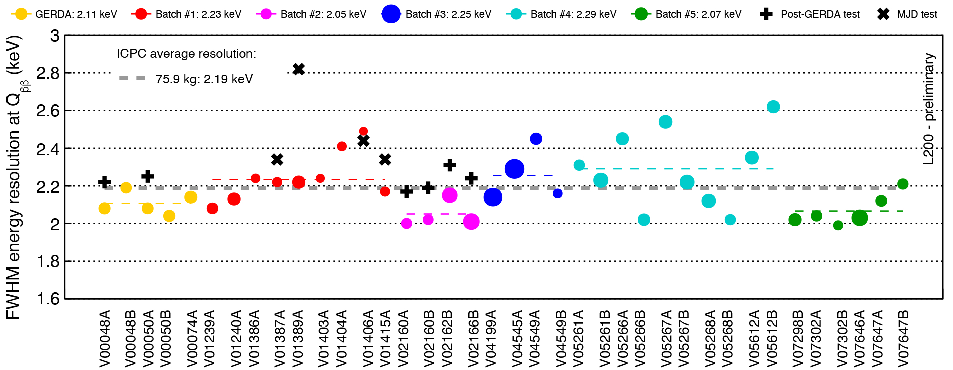
\includegraphics[width=6in]{figs/legend/icpc_resolution.pdf}
	\caption{``FWHM energy resolution of all LEGEND-200 ICPC detectors delivered to date, as measured in vendor vacuum cryostats (colored discs). The dashed lines indicate the mass-weighted average per production batch (colored) and for all detectors combined (gray). Each data point's diameter scales with its detector mass; uncertainties are on the order of or smaller than the marker sizes. Also shown are the values measured during testing in the GERDA (black plus) and {\MJDEMit} (MJD, black cross) cryostats.''~\cite{legend_pcdr}}
	\label{fig:legend_icpc_res}
\end{figure}

ICPCs have both the large mass of coaxial detectors and the low capacitance and event discrimination capabilities of point-contact detectors. Therefore, their use is integral to the LEGEND experimental strategy. L200 currently operates ICPC detectors with a mass of 1.5 - 4\,kg. The energy resolution in the vendor vacuum cryostat and relative mass of the first 5 batches of detectors to be produced for L200 is shown in Fig.~\ref{fig:legend_icpc_res}. Many of these were deployed and tested in either the {\MJDEMit} or GERDA infrastructure. While these tests show an often poorer energy resolution in the deployed state, the resolution at \Qbb{} of all except one detector test meets the 2.5\,keV FWHM goal of the LEGEND experimental program. Although encouraging, a superb energy resolution alone is insufficient to meet the performance requirements for deployment of a detector in the LEGEND experiment. Further checks are performed to determine their event discrimination capabilities during detector acceptance characterization.

\section{Detector Characterization}

All the L200 ICPCs were characterized at SURF, Oakridge National Laboratory or at the HADES underground facility in Belgium.  During detector acceptance characterization, a standard set of measurements were conducted with various radiation sources. The properties of these radiation sources were exploited to check the performance of each detector. The $^{208}$Tl 2615\,keV gamma peak present in the $^{228}$Th decay chain is well above the $2 \times 511$ keV pair production threshold. Due to their inherent topology, the double-escape and single-escape peaks of $^{208}$Tl are used as sources of predominantly single-site and multi-site events respectively. Therefore, flood (uncollimated) $^{228}$Th measurements were performed to study the single- and multi-site discrimination capabilities throughout the bulk of the detector. $^{60}$Co was used to determine the detector depletion voltage and to provide high statistics energy resolution data points which aid in the determination of the resolution at \Qbb{}.

Additional surface scans were performed to determine the detectors' n$^+$ dead layer thickness. This figure is necessary to estimate the active volume and thus effective Ge mass which feeds directly into the sensitivity calculations in Eq.~\ref{eq:Thalfexp} and Eq.~\ref{eq:Thalflim}. To determine the thickness of the dead layer a simple peak area ratio test is performed. The sub-100\,keV gamma peaks of $^{133}$Ba and $^{241}$Am are ideal for this purpose, with attenuation lengths of up to 2.2\,mm in Ge~\cite{NIST}. Note that the dead layer is around 1\,mm in depth. The number of events under the low energy peak is compared to the number of events under a higher energy peak (with attenuation length greater than the dead layer). Adjusting for the corresponding branching ratios, these values are used to determine the dead layer thickness at various locations of the detector. These surface scans are performed with collimated sources.  

The standard set of measurements performed during detector acceptance characterization provided the general performance and dead layer information needed for deployment in L200. The scope is limited by design to fit the timeframe of the experiment and minimize the exposure of enriched detectors to cosmic rays on the Earth's surface. Additionally, to minimize detector handling and contamination, measurements were performed in the vendor cryostat which restricts the sources to gamma emitters with sufficient energy to transverse the cryostat walls. However, the detector's response to alpha and beta particles is of interest given the significant contribution that alpha and beta emitters have to the background of L200 and L1000. Fortunately, natural detectors with the same geometries as those employed in LEGEND can be carefully studied without constraint. Multiple test stands were built for this purpose, including the TUBE (TUM Upside-down BEGe), GALATEA and CAGE (Collimated Alphas, Gammas, and Electrons) scanners~\cite{TUBE,GALATEA,CAGE}. These test stands require the detector to be transferred from the vendor cryostat to place alpha, beta and low-energy gamma sources next to the detector without obstruction. Due to the limited range of such particles and the use of collimated sources, the energy is deposited in a well-defined volume up to a few millimeters from the surface. Thus surface effects can be studied. For example, the TUBE scanner was used to validate the DCR discriminator employed in the {\MJDEMit}. 

The aforementioned measurements provide an incomplete picture of detector response. While flood measurements with higher-energy gamma sources (\CsS{} -- 662\,keV, $^{60}$Co -- 1173 and 1332\,keV, $^{228}$Th -- 2615\,keV) generate events throughout the bulk of the detector, pulses cannot be assigned to well-defined volumes as with surface scans. Therefore, regions of the bulk cannot be isolated and studied with this technique. Of particular interest are regions of low-electric field which are present along the long drift paths in ICPCs (see Fig.~\ref{fig:dets_efield}). Bulk charge trapping in these regions could be particularly problematic and thus the standard charge-trapping energy corrections introduced in Section~\ref{sec:charge_trapping} could fall short of accounting for uncollected charge~\cite{planar_charge_trapping}. Given the excellent performance of the ICPCs that were characterized, such effects would have to be constrained to very small volumes.  

The active volume of a detector can be estimated by comparing its intrinsic efficiency to industry standards or simulations. The intrinsic efficiency is defined as the number of FEP counts divided by the number of gamma rays incident on the detector from a flood source~\cite{knoll}. Such measurements ensure that no major dead regions exist in the detector, further constraining the volume of the hypothesized regions of problematic bulk charge trapping. 

Additional instrumentation is required to pinpoint the origin of bulk events. Doing so allows for the creation of pulse shape libraries with bulk locations assigned to each pulse shape. The power of a pulse shape library as applied to background rejection for \novbb{} searches was demonstrated by R.J. Cooper, \textit{et al.}~\cite{mjd_pulseshape_library}. In this work a basis set of single-site waveforms covering the entire bulk of a detector was generated with a prolonged $^{60}$Co flood measurement and applying an $A/E$ discriminator. The waveforms in the basis set were \textit{superpulses}, created by normalizing, aligning and averaging individual waveforms by similarity analysis to reduce noise. A background rejection algorithm was developed based on this library. The algorithm rejects a waveform if a similar waveform is not found in the basis set. With this technique 98\% \novbb-like $^{208}$Tl double escape peak events were preserved while 99\% of multi-site events in the single escape peak were rejected. Such libraries have to be created for a detector before its deployment in an experiment if this background rejection technique is to be used. Additionally, the library does not have a bulk-location assigned to each superpulse. While the former is unavoidable, an apparatus which performs the latter is introduced in the next chapter.
